%%%%%%%%%%%%%%%%%%%%%%%%%%%%%%%%%%%%
% Header                           %
%%%%%%%%%%%%%%%%%%%%%%%%%%%%%%%%%%%%
% 
% Revisions: 2017-04-10 Martin R�del <martin.raedel@dlr.de>
%                       Initial draft
%               
% Contact:   Martin R�del,  martin.raedel@dlr.de
%            DLR Composite Structures and Adaptive Systems
%          
%                                 __/|__
%                                /_/_/_/  
%            www.dlr.de/fa/en      |/ DLR
% 
%%%%%%%%%%%%%%%%%%%%%%%%%%%%%%%%%%%%
% Content                          %
%%%%%%%%%%%%%%%%%%%%%%%%%%%%%%%%%%%%

\leveldown{Preliminaries}

Generally, material models or more generelly peridynamic constitutive laws are divided by the underlying peridynamic formulation and can be grouped into two categories:

\begin{description}[noitemsep]
  \item[Bond-based] bond forces depend only on a single pair of material points
  \item[State-based] bond forces depend on deformations of all neighboring material points 
\end{description}

A rough classification of material models in \toolname{} can be found in \autoref{sec:Peridigm:QRG:Materials:Preliminaries:Classification}.

\begin{figure}[htbp]
\small
\footnotesize
\centering
%%%%%%%%%%%%%%%%%%%%%%%%%%%%%%%%%%%%
% Header                           %
%%%%%%%%%%%%%%%%%%%%%%%%%%%%%%%%%%%%
% 
% Revisions: 2017-04-10 Martin Raedel <martin.raedel@dlr.de>
%                       Initial draft
%               
% Contact:   Martin Raedel,  martin.raedel@dlr.de
%            DLR Composite Structures and Adaptive Systems
%          
%                                 __/|__
%                                /_/_/_/  
%            www.dlr.de/fa/en      |/ DLR
% 
%%%%%%%%%%%%%%%%%%%%%%%%%%%%%%%%%%%%
% Content                          %
%%%%%%%%%%%%%%%%%%%%%%%%%%%%%%%%%%%%

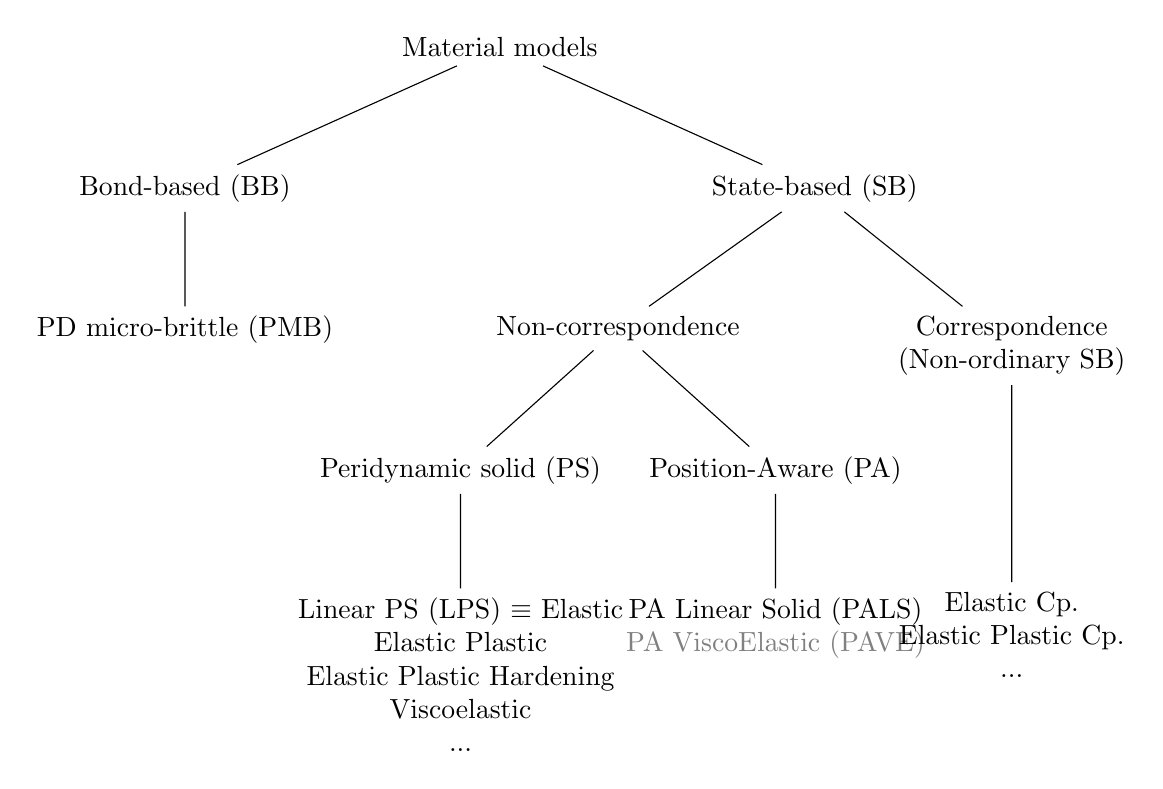
\begin{tikzpicture}[
% for small:
% for footnotesize:
  basic/.style = {anchor=north},
  level distance=1.5cm,
  level 1/.style={basic,sibling distance=8cm},
  %level 2/.style={basic,sibling distance=6cm},
  level 2/.style={basic,sibling distance=5cm},
  %level 3/.style={basic,sibling distance=5.0cm},
  level 3/.style={basic,sibling distance=4.0cm},
  level 4/.style={basic,sibling distance=1.75cm},
  level 5/.style={basic,sibling distance=1.0cm},
  %growth parent anchor = north,
]
  \node {Material models}
    child {node {Bond-based (BB)}
      %child {node {Peridynamic micro-brittle (PMB)}}
      child {node {PD micro-brittle (PMB)}}
    }
    child {node {State-based (SB)}
      child {node {Non-correspondence}
        child {node {Peridynamic solid (PS)}
          child {node[align=center] {%
            Linear PS (LPS) $\equiv$ Elastic\\%
            Elastic Plastic\\%
            Elastic Plastic Hardening\\%
            Viscoelastic\\%
            ...%
          }}
        }
        child {node {Position-Aware (PA)}
          child {node[align=center] {%
            %Position-Aware Linear Solid (PALS)\\%
            %\textcolor{gray}{Position-Aware ViscoElastic (PAVE)}%
            PA Linear Solid (PALS)\\%
            \textcolor{gray}{PA ViscoElastic (PAVE)}%
          }}
        }
      }
      child {node[align=center] {Correspondence\\(Non-ordinary SB)}
        child {%node {}
          child {node[align=center] {%
            Elastic Cp.\\%
            Elastic Plastic Cp.\\%
            ...%
          }}
        }
      }
    };
\end{tikzpicture}
\caption{Classification of peridynamic material models}
\label{sec:Peridigm:QRG:Materials:Preliminaries:Classification}
\end{figure}

Bond-based material models are not discussed here any further. Peridynamic state-based material models are further divided in two main classes, the 

\begin{itemize}[noitemsep]
  \item non-correspondence and
  \item correspondence
\end{itemize}

materials. The non-correspondence is material created directly in the peridynamic formulation. The correspondence material is formulated in the classical continuum mechanical way. Both material classes will/should evaluate the same result for the same material modeled if surface effects have no influence. However, the correspondence material gives additional outputs as Cauchy stresses. This makes the results more comparable to the standard formulation.

\leveldown{Comments on non-correspondence material models}
\label{sec:Peridigm:QRG:Materials:Preliminaries:NonCorrespondence}

\leveldown{Description}

There are sub-classes of non-correspondence material models. The first material model implementation is the peridynamic micro-brittle (PMB) material for bond-based peridynamics. Due to the limitations of bond-based peridynamics, this is not further discussed here.

State-based non-correspondence material models are the linear peridynamic solid (LPS) model and its extension to other types of material behaviour, like plasticity or viscoelasticity. These materials suffer from one large disadvantage, the underlying mathematical models assume that all points within are in the bulk. However, points near the surface are missing bonds. Missing bonds imply and induce incorrect material properties. Thus, these models are consistent.

To overcome this limitation, the so-called \textit{Position-Aware} class of material models was developed.

\levelstay{Remarks}

\begin{itemize}[noitemsep]
  \item If not stated otherwise, peridynamic solid non-correspondence (PS) materials in \toolname{} do not have surface correction implemented.
  \item Position-aware (PA) materials were developed to account for missing bonds on surfaces removing the need for auxiliary surface correction techniques.
\end{itemize}


\levelup{Comments on correspondence material models}
\label{sec:Peridigm:QRG:Materials:Preliminaries:Correspondence}

\begin{itemize}[noitemsep]
  \item Do not require surface correction
  \item Might suffer from zero-energy modes
  \item Each family needs at least 3 non-collinear bonds active, otherwise the deformation gradient can not be calculated and the solution fails.
  \item Therefore, the bond check algorithm included in the interface aware damage model (cf. section \ref{sec:Peridigm:QRG:Damage:InterfaceAware}) has to be included if a damage model should be used.
\end{itemize}